\documentclass[11pt]{article}
\usepackage[a4paper,includeheadfoot,margin=2.54cm]{geometry}
\usepackage[T2A]{fontenc}
\usepackage[utf8]{inputenc}
\usepackage[bulgarian]{babel}
\usepackage[unicode=true]{hyperref}
\usepackage{breakurl}
\usepackage{indentfirst}
\usepackage{pgf, tikz}
\usepackage{amsmath}
\usepackage{amsthm}
\usepackage{amssymb}
\usepackage{mathtools}
\usepackage{esvect}
\usepackage{breqn}

\usepackage{graphicx}
\graphicspath{ {image/} }

\numberwithin{equation}{section}
\numberwithin{figure}{section}
\numberwithin{table}{section}
  \theoremstyle{plain}
  \newtheorem{thm}{\protect\theoremname}[section]
  \theoremstyle{definition}
  \newtheorem{defn}[thm]{\protect\definitionname}
  \theoremstyle{remark}
  \newtheorem*{notation*}{\protect\notationname}
  \theoremstyle{definition}
  \newtheorem*{example*}{\protect\examplename}
  \theoremstyle{remark}
  \newtheorem*{note*}{\protect\notename}
  \theoremstyle{plain}
  \newtheorem{lem}[thm]{\protect\lemmaname}
  \theoremstyle{definition}
  \newtheorem*{defn*}{\protect\definitionname}
  \theoremstyle{definition}
  \newtheorem{example}[thm]{\protect\examplename}
  \theoremstyle{plain}
  \newtheorem{cor}[thm]{\protect\corollaryname}
  \theoremstyle{plain}
  \newtheorem{prop}[thm]{\protect\propositionname}
  \theoremstyle{plain}
  \newtheorem*{prop*}{\protect\propositionname}
  \theoremstyle{definition}
  \newtheorem{xca}[thm]{\protect\exercisename}
  \newcommand\thmsname{\protect\theoremname}
%  \newcommand\nm@thmtype{theorem}
  \theoremstyle{plain}
  \newtheorem*{namedtheorem}{\thmsname}
  \newenvironment{namedthm}[1][Undefined Theorem Name]{
   \ifx{#1}{Undefined Theorem Name}\renewcommand\nm@thmtype{theorem*}
   \else\renewcommand\thmsname{#1}\renewcommand\nm@thmtype{namedtheorem}
   \fi
   \begin{\nm@thmtype}}
   {\end{\nm@thmtype}}

  \providecommand{\corollaryname}{Следствие}
  \providecommand{\definitionname}{Дефиниция}
  \providecommand{\examplename}{Пример}
  \providecommand{\exercisename}{Упражнение}
  \providecommand{\lemmaname}{Лема}
  \providecommand{\notationname}{Нотация}
  \providecommand{\notename}{Забележка}
  \providecommand{\propositionname}{Твърдение}
  \providecommand{\remarkname}{Забележка}
  \providecommand{\theoremname}{Теорема}

\DeclarePairedDelimiter\norm{\lVert}{\rVert}
\renewcommand*{\Vec}[1]{\mathbf{#1}}
\newcommand*{\Z}{\Vec{0}}
\newcommand*{\B}{\mathcal{B}}
\newcommand*{\R}{\mathbb{R}}

\title{Лекционни записки по Математически Анализ}
\author{проф. Надежда Рибарска \\ Набрани от Никола Юруков}
\date{\today}


\begin{document}

\maketitle

\clearpage

\tableofcontents

\clearpage

\section{Лекция 1 - преговор с разширение}

\subsection{Евклидовото пространство $\mathbb{R}^n$}

Като множество $\mathbb{R}^n$ е множеството $\{x = (x_1, x_2, ..., x_n): x_i \in \mathbb{R}, \  i=1,2,..,n\}$ от нередените $n$-торки реални числа. Ако го снабдим със стандартните линейни операции събиране на вектори и умножение на вектор с реално число, получаваме реално линейно пространство (спомнете си аксиомите от курса по линейна алгебра). Да напомним формалните дефиниции: сума на векторите $x = (x_1, x_2, ..., x_n)$ и $y = (y_1, y_2, ..., y_n)$ е векторът $x+y = (x_1+y_1, x_2+y_2, ..., x_n + y_n)$ (събирането е покоординатно). Произведение на скалара $\lambda \in \mathbb{R}$ с вектора $x$ е векторът $\lambda x = (\lambda x_1, \lambda x_2, ..., \lambda x_n)$ (умножението със скалар също е покоординатно). Ще означаваме с $\Z$ нулевия вектор $(0,\dots ,0)$.

За да можем да правим анализ (да говорим за граница, непрекъснатост, производна и т.н.), освен линейната структура ни е необходима и някаква "мярка на близост" в нашето пространство. Както помните от курса по ДИС2, стандартната мярка на близост  между два вектора е евклидовото разстояние между тях:
 $$\rho(x,y):= \sqrt{\sum_{i=1}^n (x_i-y_i)^2} \ , \mbox{ където } x = (x_1, x_2, ..., x_n), \ y = (y_1, y_2, ..., y_n) \ .$$
 Забележете, че в $\mathbb{R}^2$ това е просто питагоровата теорема. Това разстояние е добре съгласувано с линейната структура в смисъл, че $\rho(x,y)=\lVert x - y\rVert$, където в дясната част стои евклидовата норма (или дължината) на вектора $x-y$:
 $$\lVert x\rVert := \sqrt{\sum_{i=1}^n x_i^2}\ , \ x = (x_1, x_2, ..., x_n) \ .$$

 Да напомним, че една функция $\lVert \cdot \rVert :\mathbb{R}^n \longrightarrow [0,+\infty)$ се нарича норма, ако за нея са в сила свойствата
\begin{enumerate}
	\item $\lVert x \rVert = 0 \iff x=\Z$
	\item $\norm{\lambda x} = |\lambda|\cdot \norm{x}$
	\item $\norm{x+y} \leq \norm{x} + \norm{y}$ (неравенство на триъгълника)
\end{enumerate}

В курса по ДИС2 е проверено, че евклидовата норма е норма. За упражнение проверете, че
\begin{itemize}
 \item $\norm{(x_1, x_2)}_1 = |x_1| + |x_2|$
 \item $\norm{(x_1, x_2)}_\infty = $ max\{$|x_1|, |x_2|$\}
 \item $\norm{(x_1, x_2)}_p = \sqrt[p]{|x_1|^p + |x_2|^p}$, $1< p<\infty$
\end{itemize}
са норми в $\mathbb{R}^2$.
По-общо, проверете, че  $$\norm{x}_p = \sqrt[p]{\sum_{i=1}^n |x_i|^p} \ , \ 1\leq p<\infty \mbox{ е норма в } \mathbb{R}^n \ .$$
Разбира се, за целта трябва да използвате неравенството на Минковски от курса по ДИС2.

Евклидовата норма има по-хубави геометрични свойства от горните примери, защото е съгласувана със скаларното произведение
$$\langle x, y\rangle = \sum_{i=1}^n x_i y_i  \ , \mbox{ където } x = (x_1, x_2, ..., x_n) \mbox{ и } \ y = (y_1, y_2, ..., y_n),$$
по стандартния начин $\lVert x \rVert =\sqrt{\langle x, x\rangle}$. Да напомним основното неравенство на Коши-Буняковски-Шварц:
$$|\langle x, y\rangle | \leq \norm{x}\norm{y} \ .$$

Да напомним също означенията
$$B_r(x) := \left\{ y\in \mathbb{R}^n : \norm{y-x}<r\right\}$$
за отворено кълбо с център $x$ и радиус $r$ и
$$\overline{B}_r(x) := \left\{ y\in \mathbb{R}^n : \norm{y-x}\leq r\right\}$$
за затворено кълбо с център $x$ и радиус $r$. Като упражнение можете да скицирате кълбата с радиус 1 и център началото на координатната система за нормите $\norm{\cdot}_1$ и $\norm{\cdot}_\infty$ от предишното упражнение.

%TODO add graphics for intervals and p-norms.

\subsection{Топология в $\mathbb{R}^n$}

\begin{defn}
Подмножеството $U$ на $\R^n$ се нарича отворено, ако за всяка точка $x$ от $U$ съществува $\varepsilon>0$ такова, че $B_\varepsilon (x) \subset U$.
\end{defn}

Основните свойства на отворените множества, проверени в курса по ДИС2, са

1. $\emptyset$ и $\R^n$ са отворени

2. Сечение на краен брой отворени множества е отворено, т.е. ако $U_1, U_2, ..., U_k$ са отворени, то $\bigcap_{i=1}^k U_i$ е отворено.

3. Обединение на произволна фамилия от отворени множества е отворено, т.е. ако $U_\alpha$ са отворени за всяко $\alpha \in I$, то $\bigcup _{\alpha \in I} U_\alpha$ е отворено.

\begin{example}
Отворените кълба са отворени множества.
\begin{proof}
Да разгледаме $B_r(x_0)$, $r>0$. Взимаме си произволно $x$ от кълбото, т.е. растоянието между $x$ и $x_0$ е по-малко от $r$. Нека $\varepsilon := r - \norm{x_0-x}>0$. Тогава $B_\varepsilon(x)\subset B_r(x_0)$. Наистина, нека $y\in B_\varepsilon(x)$, т.е. $\norm{y-x} <\varepsilon$. Получаваме
\begin{eqnarray*}
\norm{x_0-y} &\leq& \norm{x-y} + \norm{x-x_0} < \varepsilon + \norm{x-x_0}\\
\norm{x_0-y} &<& r - \norm{x_0-x} + \norm{x-x_0}\\
\norm{x_0-y} &<& r
\end{eqnarray*}
\end{proof}
\end{example}

\begin{example}
Нека функцията  $g:\R^n \rightarrow \R$ е \textbf{непрекъсната}. Тогава множеството \\ $U = \{x\in\R^n:g(x)>0\}$ е отворено.
\begin{proof}
Взимаме произволна точка $x_0\in U$, следователно $\varepsilon = g(x_0)>0$. От непрекъснатостта на функцията получаваме, че съществува положително число $\delta$ такова, че $|g(x)-g(x_0)|<\varepsilon$ за всяко $x\in B_\delta(x_0)$. Следователно $g(x)>g(x_0)-\varepsilon = 0$ и оттук $x \in U$ за всяко $x\in B_\delta(x_0)$.
\end{proof}
\end{example}

\begin{defn} Едно подмножество
$F$ на $\R^n $ се нарича затворено, ако $\R^n \setminus F$ е отворено множество.
\end{defn}

Основните свойства на затворените множества, проверени в курса по ДИС2, са

1. $\emptyset, \R^n$ са затворени.

2. Обединие на краен брой затворени множества е затворено, т.е. ако $F_1, F_2, ..., F_k$ са затворени, то $\bigcup_{i=1}^k F_i$ е затворено.

3. Сечение на произволна фамилия от затворени множества е затворено, т.е. ако $F_\alpha$ са затворени за всички $\alpha \in I$, то $\bigcap _{\alpha \in I} F_\alpha$ е затворено.

\begin{example}
Затворените кълба са затворени множества. Доказателството оставяме за упражнение.
\end{example}

\begin{defn}
Контур на множеството $A \subset \R^n$ наричаме множеството
$$\partial A := \{ x\in \R^n : \forall U \; \text{отворено}, \; x\in U \mbox{ е в сила } U \cap A \neq \emptyset \mbox{ и } U\setminus A \neq \emptyset \}$$
\end{defn}

\begin{defn}
Затворена обвивка на множеството $A \subset \R^n$ наричаме най-малкото затворено множество, съдържащо $A$:
$$\overline{A} := \cap \left\{ F \subset \R^n : \ F \supset A  \mbox{ и } F  \mbox{ е затворено }\right\}$$
\end{defn}

В курса по ДИС2 е доказано, че
$$\overline{A} = \{x\in\R^n: \exists \{x_m\}_{m=1}^\infty \subset A,\; x_m \rightarrow x \}$$
Лесно се проверява, че едно множество е затворено точно тогава, когато съвпада със затворената си обвивка. Връзките между контур на множество и затворена обвивка на множество са
$$\overline{A}= A \cup \partial A \ , \ \partial A =\overline{A} \cap \left(\overline{\R^n\setminus A}\right) \ .$$
Следователно контурът на произволно множество е винаги затворено множество. Също лесно се проверява, че
$$\partial A = \{x \in \R^n : \ \exists \{x_m\}_{m=1}^\infty \subset A, \ x_m \rightarrow x  \mbox{ и } \exists \{y_m\}_{m=1}^\infty \subset \R^n\setminus A, \  y_m \rightarrow x\}$$

\begin{defn}
Вътрешност на $A\subset\R^n$ наричаме най-голямото отворено множество, съдържащо се в $A$:
$$\mathring{A} = \cup \left\{ U \subset \R^n : \ U \subset A  \mbox{ и } U  \mbox{ е отворено }\right\}$$
\end{defn}

Друго означение за вътрешност на $A$ е $int A$. Понятието за вътрешност е дуално на понятието за затворена обвивка, т.е.
$$int{A} = \R^n \setminus \left(\overline{\R^n\setminus A}\right) \ , \ \overline{A}=
\R^n \setminus \left(int{(\R^n\setminus A)}\right) \ .$$

Едно от най-важните и често използвани понятия в топологията е понятието за компактност.
\begin{defn}
Едно множество $A\subset \R^n$ се нарича компакт, ако от всяко негово отворено покритие можем да изберем крайно подпокритие, т.е. ако $\{U_\alpha\}_{\alpha \in I}$ е фамилия от отворени подмножества на $\R^n$, за която е в сила $\cup_{\alpha\in I} U_\alpha \supset A$, то можем да изберем краен брой индекси $\alpha_1, \alpha_2, \dots , \alpha_k \in I$ такива, че $\cup_{i=1}^k U_{\alpha_i} \supset A$.
\end{defn}

В курса по ДИС2 са доказани две важни и нетривиални характеризации на компактните подмножества на $\R^n$:

1. Едно подмножество $A$ на $\R^n$ е компакт точно тогава, когато $A$ е ограничено и затворено.

2. Едно подмножество $A$ на $\R^n$ е компакт точно тогава, когато от всяка редица от негови елементи може да се избере сходяща подредица, чиято граница е също в множеството.

\bigskip

Сега въвеждаме първото разширение, т.е. понятие, за което не сте учили в курса по ДИС2: множество, релативно отворено в $A$. Ще го използваме по-нататък, за да говорим за множества, релативно отворени в някаква гладка двумерна повърхнина в тримерното евклидово пространство. Интуицията е, че забравяме за всичко извън множеството $A$.

\begin{defn} Нека $A \subset \R^n$. Едно подмножество $U$ на $A$ наричаме релативно отворено в $A$, ако съществува отворено множество $V\subset \R^n$ такова, че $U = A\cap V$.
\end{defn}
\begin{prop}
Множеството $U\subset A$ е релативно отворено в $A$ точно тогава, когато за всяка негова точка $x\in U$ съществува $\varepsilon >0$ такова, че $B_\varepsilon (x)\cap A \subset U$.
\end{prop}
\begin{proof}
Нека първо $U\subset A$ е релативно отворено в $A$ и $x\in U$ е произволна. Тогава съществува отворено множество $V\subset \R^n$ с $U = A\cap V$. Тъй като $x\in U\subset V$, съществува $\varepsilon >0$ с $B_\varepsilon (x) \subset V$ и оттук $B_\varepsilon (x)\cap A \subset V\cap A=U$. В обратната посока, нека за всяка точка $x\in U$ съществува $\varepsilon_x >0$ такова, че $B_{\varepsilon_x} (x)\cap A \subset U$. Полагаме
$V:= \cup_{ x\in U} B_{\varepsilon_x} (x)$. Очевидно $V$ е отворено множество като обединение на отворени кълбета. Освен това
$$V\cap A=\left(\cup_{ x\in U} B_{\varepsilon_x} (x)\right)\cap A=\cup_{ x\in U}\left( B_{\varepsilon_x} (x)\cap A\right)\subset U \ .$$
От друга страна, всяка точка $x\in U$ принадлежи на $B_{\varepsilon_x} (x) \subset V$, следователно $U\subset V$ и от $U\subset A$ следва $U\subset V\cap A$. С това $U= V\cap A$ и доказателството е завършено.
\end{proof}

Следното приложение на понятието за релативна отвореност е важно и изключително често използвано:
\begin{prop}
Нека $f: D \longrightarrow \R^m$ е изображение с дефиниционна област $D\subset \R^n$ и стойности в $\R^m$. Твърдим, че $f$ е непрекъсната в $D$ точно тогава когато първообраз на всяко отворено в $\R^m$ множество е релативно отворено в $D$. Да напомним, че първообраз на $U\subset \R^m$ е множеството
$f^{-1} (U) := \{x\in D: f(x) \in U\}$.
\end{prop}
\begin{proof}
Първо ще докажем, че ако първообраз на всяко отворено в $\R^m$ множество е релативно отворено в $D$, то $f$ е непрекъсната.
Избираме произволна точка $x$ от $D$ и произволно $\varepsilon >0$. Тъй като кълбото $B_{\varepsilon}(f(x))$ е отворено в $\R^m$, първообразът $f^{-1} (B_{\varepsilon}(f(x)))$ ще е релативно отворен в $D$. Тогава $f^{-1} (B_{\varepsilon}(f(x)))= D \cap V$ за някое множество $V$, отворено в $\R^n$. Тъй като $x\in f^{-1} (B_{\varepsilon}(f(x)))\subset  V$, съществува $\delta >0$ с $B_\delta (x) \subset V$. Нека $x'\in D$ е произволна точка с $\| x' -x\| <\delta$. Значи $x' \in D \cap B_\delta(x) \subset D\cap V=f^{-1} (B_{\varepsilon}(f(x)))$ и следователно $f(x')\in B_{\varepsilon}(f(x))$, т.е. $\| f(x')-f(x)\| <\varepsilon$.

За да докажем обратната посока, избираме произволно отворено $U\subset \R^m$.
Нека $x\in f^{-1} (U)$. Тогава $f(x)$ принадлежи на отвореното множество $U$ и следователно съществува $\varepsilon >0$ такова, че $B_\varepsilon(f(x)) \subset U$. Тъй като $f$ е непрекъсната в $x$, съществува $\delta >0$ такова, че $\| f(x')-f(x)\| <\varepsilon$ за всяко $x'\in D$, за което $\| x'-x\| <\delta$. Записано по друг начин това означава, че $f(B_{\delta}(x)\cap D) \subset B_\varepsilon (f(x)) \subset U$, следователно $B_{\delta}(x)\cap D \subset f^{-1} (U)$. Така доказахме, че множеството $f^{-1} (U)$ е релативно отворено в $D$, защото изпълнява условието от предишното твърдение.
\end{proof}

\subsection{Основни теореми}

\begin{thm}[Теорема на Вайерщрас]
Непрекъснат образ на компакт е компакт. Формално записано, ако
$f: K  \longrightarrow \R^m$ е непрекъснато изображение с дефиниционна област компактното подмножество $K$ на $\R^n$, то множеството  $f(K) := \{f(x):x\in K\}$ от стойностите на $f$ е компактно подмножество на $\R^m$.
\end{thm}
\begin{proof}
Нека $\{y_l\}_{l=1}^\infty \subset f(K)$ е редица от елементи на $f(K)$. Тогава за всеки елемент $y_l$ на тази редица съществува елемент  $x_l$ на $K$ такъв, че $y_l = f(x_l)$. Сега редицата $\{x_l\}_{l=1}^\infty$ се съдържа в компактното множество $K$. Следователно съществува нейна сходяща подредица $\{ x_{l_k}\}_{k=1}^\infty$, чиято граница $x_0$ е елемент на $K$. Тъй като $f$ е непрекъсната, от дефиницията на Хайне за непрекъснатост получаваме, че $f(x_{l_k}) = y_{l_k} \xrightarrow[k \rightarrow \infty]{} f(x_0)$. Тъй като очевидно $f(x_0)\in f(K)$, остава да се позовем на характеризацията (2) на компактните множества.
\end{proof}

Хубаво упражнение е да се докаже теоремата на Вайерщрас, като се използва дефиницията на компакт и характеризацията на непрекъснатите изображения, която доказахме.

Друго добро упражнение е да се убедите, че теоремата на Вайерщрас от ДИС 1 (една непрекъсната функция върху краен затворен интервал е ограничена и достига своята най-голяма и най-малка стойност) е следствие от тази форма на теоремата.

\bigskip

\begin{thm}[Теорема на Кантор]
Нека $f:D\longrightarrow \R^m$ е дефинирана в $D \subset \R^n$. Нека $K$ е компактно подмножество на $D$.
Ако $f$ е непрекъсната в $K$, т.е. непрекъсната е във всяка точка от $K$, то твърдим, че за всяко
$\varepsilon >0$ съществува $\delta >0$ такова, че за всяко $x \in K$ и за всички $x' \in D$, за които е изпълнено $\norm{x'-x}<\delta$, е в сила
$\|f(x)-f(x')\|<\varepsilon$. Забележете, че заключението е малко по-силно от равномерна непрекъснатост на $f$ върху $K$.
\end{thm}
\begin{proof}
Отново ще използваме характеризацията (2) на компактността чрез редици. Допускаме противното, т.е. съществува такова $\varepsilon_0 >0$, че за всички $\delta >0$ съществуват точки $x_\delta \in K$ и $x'_\delta \in D$ такива, че
$$\norm{x_\delta - x'_\delta}<\delta \mbox{ и } \|f(x_\delta)-f(x'_\delta)\|\geq \varepsilon \ .$$
Даваме на $\delta$ стойности  $1, \frac{1}{2}, \frac{1}{3}, \dots$ и преименуваме $x_{1/m}$ и $x_{1/m}'$ съответно на $x_m$ и $x'_m$. Така се образуват две редици $\{x_m\}_{m=1}^\infty \subset K$ и $\{x'_m\}_{m=1}^\infty \subset D$.
Знаем, че
$$\norm{x_m - x'_m}<\frac{1}{m} \mbox{ и } \|f(x_m) - f(x'_m)\|\geq \varepsilon_0 >0$$
за всяко естествено $m$. Тъй като $K$ е компакт, съществува сходяща подредица $x_{m_k} \xrightarrow[k \rightarrow \infty]{} x_0 \in K$ на $\{x_m\}_{m=1}^\infty \subset K$. От неравенствата
$$\norm{x'_{m_k}-x_0}\leq \norm{x'_{m_k}-x_{m_k}} + \norm{x_{m_k} - x_0} < \frac{1}{m_k} + \norm{x_{m_k}-x_0}$$
получаваме, че редицата $\{x'_{m_k}\}_{k=1}^\infty$ също клони към точката $x_0\in K$. Сега използваме непрекъснатостта
на $f$ в точката $x_0\in K$ и получаваме, че
$$f(x_{m_k}) \xrightarrow[k \rightarrow \infty]{} f(x_0)\mbox{ и } f(x_{m_k}') \xrightarrow[k \rightarrow \infty]{} f(x_0) .$$
Като извадим тези две редици, получаваме
$f(x_{m_k}) - f(x'_{m_k}) \xrightarrow[k \rightarrow \infty]{} 0$, което противоречи на $\|f(x_m) - f(x'_m)\|\geq \varepsilon_0 >0$ за всяко естествено $m$. Теоремата е доказана.
\end{proof}

\section{Лекция 2. Кратен Риманов интеграл - въвеждане и основни свойства}

Конструкцията на Дарбу, с която сте въвели Риманов интеграл в курса по ДИС1, е важна и естествена и ние ще я използваме отново, за да въведем $n$-кратен Риманов интеграл. Геометричната интуиция остава същата. В курса по ДИС1 сте искали да дефинирате по един разумен начин лицето на фигура, заградена от абцисата, две вертикални прави и графиката на ограничена неотрицателна функция. Постигнали сте го чрез оценяване отгоре и отдолу на това лице чрез лицата на стъпаловидни фигури, съставени от краен брой правоъгълници (тези лица са големите и малките суми на Дарбу). Сега за $n$=2 трябва да оценяваме отгоре и отдолу обема на тяло, заградено от равнината на първите две координатни оси, вертикални равнини по границата на даден правоъгълник и графиката на ограничена неотрицателна функция, дефинирана в този правоъгълник. Оценката е чрез обема на тела, състоящи се от краен брой паралелепипеди (за оценка отгоре вземаме обема на такова стъпаловидно тяло, съдържащо нашето, а за оценка отдолу - съдържащо се в нашето). За по-големи размерности идеята и конструкцията остават същите, само че вече не можем да нарисуваме подходяща картинка.

\subsection{Паралелотопи в $\R^n$ и тяхната мярка}

Първият въпрос, който трябва да решим, е с какво заменяме крайния и затворен интервал от ДИС1, ако размерността е по-голяма от едно. Естественият отговор е: с правоъгълник в равнината, с паралелепипед в тримерното пространство и т.н.

\begin{defn}
Паралелотоп (на английски interval, box) е множество в $\R^n$, за което всяка координата се мени (независимо от останалите) в краен затворен интервал:
$$\Delta := \{x\in\R^n : a_i \leq x_i \leq b_i,\; i = 1, 2, ... n \} \ .$$
\end{defn}

За различните размерности (стойности на $n$) имаме

\begin{tabular}{ c l }
  $n$ & \multicolumn{1}{c}{$\Delta$}\\
  \hline
  1 & $[a_1, b_1]$ \mbox{ интервал }\\
  2 & $[a_1, b_1]\times[a_2, b_2]$ \mbox{ правоъгълник }\\
  3 & $[a_1, b_1]\times[a_2, b_2]\times[a_3, b_3]$\mbox{ паралелепипед }\\
  ..& ...
\end{tabular}

Същественото за тези най-прости фигури е, че нямаме съмнения какво трябва да наречем дължина на интервал, лице на правоъгълник, обем на паралелепипед, а за паралелотоп в $\R^n$ естествено въвеждаме мярка в $\R^n$.

\begin{defn}
За паралелотопа $\Delta = \{x\in\R^n : a_i \leq x_i \leq b_i,\; i = 1, 2, ... n \}$ дефинираме неговата $n$-мерна мярка като
$$\mu_n(\Delta) := \prod_{i=1}^n (b_i - a_i) \ .$$
\end{defn}

Забележете, че при $n=1$ това е дължината $\mu_1([a_1,b_1]) = b_1 - a_1$ на интервала $[a_1,b_1]$, при $n=2$ това е лицето $\mu_2([a_1,b_1]\times [a_2,b_2]) = (b_1 - a_1)(b_2-a_2)$ на правоъгълника $[a_1, b_1]\times[a_2, b_2]$, при $n=3$ това е обемът $\mu_3([a_1, b_1]\times[a_2, b_2]\times[a_3, b_3]) = (b_1 - a_1)(b_2-a_2)(b_3-a_3)$ на паралелепипеда $[a_1, b_1]\times[a_2, b_2]\times[a_3, b_3]$.


\bigskip

Следващият етап е да уточним как да разделяме паралелотоп на паралелотопчета по аналогия с разделянето на интервал на подинтервали от ДИС1. Неформално, подразделяне на паралелотоп са краен брой паралелотопи, чието обединение е първоначалният паралелотоп, и които не се припокриват.

\begin{defn}
Подразделение $\Pi$ на един паралелотоп $\Delta$ е крайно множество от паралелотопи
$\Pi = \{\Delta_k \}_{k=1}^{k_0}$, за което
 $\cup_{k=1}^{k_0} \Delta_k = \Delta$ и $\mathring \Delta_{k} \cap \mathring \Delta_{l} = \emptyset \; \forall k \neq l$.
\end{defn}

\begin{center}
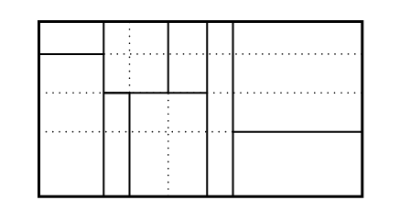
\includegraphics[scale=0.5]{rectangle-subdivision}
\end{center}

Забележете, че вътрешността на паралелотопа $\Delta = \{x\in\R^n : a_i \leq x_i \leq b_i,\; i = 1, 2, ... n \}$ е множеството $\mathring \Delta = \{x\in\R^n : a_i < x_i < b_i, \; i=1,2,..n\}$. Следното твърдение е геометрически очевидно, но съществено за по-нататъшната ни работа:

\begin{prop}
Ако $\Pi = \{\Delta_k \}_{k=1}^{k_0}$ е подразделяне на $\Delta$, то $\mu_n(\Delta) = \sum_{k=1}^{k_0} \mu_n(\Delta_k)$.
\end{prop}

\begin{proof}
Първо разглеждаме случая на правилно подразделяне, т.е. $\Pi$ се получава като се раздели интервалът, в който се мени $i$-тата координата, на подинтервали за всяко $i$, и се вземат всевъзможните декартови произведения на такива подинтервали.
За пестене на място и по-прости означения ще изпишем нещата за $n=2$, в общия случай доказателството е аналогично. И тъй, нека
$\Delta =[a_1,b_1]\times [a_2,b_2]$ и делим $[a_1,b_1]$ и $[a_2,b_2]$ на подинтервали:
$$a_1 = x_0 < x_1 < ... < x_{m_0} = b_1 \ ,$$
$$a_2 = y_0 < y_1 < ... < y_{l_0} = b_2 \ .$$
Тогава $\Pi = \{\Delta_{m l} : \ m=1,\dots ,m_0, \ l=1, \dots ,l_0\}$, където 
$\Delta_{m l} = [x_{m-1}, x_m]\times [y_{l-1}, y_l]$. Пресмятаме
\begin{dmath*}
\sum_{l=1}^{l_0} \sum_{m=1}^{m_0} \mu_2 (\Delta_{m l}) = \sum_{l=1}^{l_0} \sum_{m=1}^{m_0} (x_m - x_{m-1})(y_l - y_{l-1}) = \sum_{l=1}^{l_0} (y_l - y_{l-1})\sum_{m=1}^{m_0} (x_m - x_{m-1}) = (b_1 - a_1) \sum_{l=1}^{l_0}(y_l - y_{l-1}) = (b_1 - a_1) (b_2 - a_2) = \mu_2(\Delta)
\end{dmath*}

Нека сега да разгледаме произволно подразделяне $\Pi = \{\Delta_k \}_{k=1}^{k_0}$. Можем да намерим правилно подразделяне $\Pi^*$ на $\Delta$ такова, че елементите на $\Pi^*=\{\Delta_l^* \}_{l=1}^{l_0}$, които се съдържат в $\Delta_k$, образуват подразделяне на $\Delta_k$ (например при размерност 2 продължаваме вертикалните и хоризонтални страни на правоъгълниците от $\Pi$ в целите интервали). Тогава, използвайки два пъти предишната стъпка, получаваме 
$$\mu_n(\Delta) = \sum_{l=1}^{l_0} \mu_n(\Delta_l^*)= \sum_{k=1}^{k_0} \left(\sum_{\Delta_l^*\subset \Delta_k} \mu_n(\Delta_l^*)\right)=\sum_{k=1}^{k_0} \mu_n(\Delta_k) \ .$$
\end{proof}

%Така ...


\end{document} 